\addbibresource{reference.bib}

\chapter{Úvod}\label{chap01} 
Tato diplomová práce se zabývá návrhem a implementací softwarového systému \textbf{Pixnet} - software pro distribuované řízení sítě částicových pixelových detektorů. Software byl navržen především pro řízení detektorů \textit{Timepix3}, ale díky modulární architektuře (po implementaci potřebných modulů) je možné ho použít na řízení libovolného detektoru.

Systém se skládá z několika částí - backendové aplikace \textbf{handleru} (software pro řízení a vyčítání dat z jemu přiřazených detektorů - viz kapitola \ref{chap:handler}), backendové aplikace \textbf{mastera} (software pro řízení sítě handlerů - viz \ref{chap:master:backend}) a frontendové webové \textit{single-page} aplikace \textbf{mastera} (software poskytující webové uživatelské rozhraní pro řízení mastera pomocí jeho API - viz \ref{chap:master:frontend}).

V rámci této práce byly implementovány moduly, které systému Pixnet umožňují řízení a vyčítání dat z detektorů \textit{Timepix3}, připojeným pomocí vyčítacího rozhraní \textit{Katherine}, viz kapitola \ref{chap:katherine}.

\section{Motivace}
Podobný systém pro řízení sítě částicových pixelových detektorů již existuje \cite{atlastpx_sw,BegeraBcThesis2016} a byl vyvinut pro účely řízení a vyčítání dat z experimentu \textit{ATLAS-TPX} - sítě \textit{Timepix} detektorů, která byla instalována v rámci experimentu \textit{ATLAS} na \textit{LHC} v \textit{CERN} a měřila data během \textit{LHC} \texttt{run 2}\footnote{Označení druhého běhu částicového urychlovače \textit{LHC}, který probíhal v letech 2014 až 2018.}. 

V letech 2019 až 2020 je plánován LS2\footnote{Z angl. \textit{Long Shutdown 2}, technologická odstávka částicového urychlovače \textit{LHC}.}, v rámci které proběhne modernizace detektorové sítě \textit{ATLAS-TPX} za použití detektorů \textit{Timepix3}. Z pohledu softwarové architektury modernizace přináší nová omezení, které existující systém není schopný zajistit. Především se jedná o vysoký datový tok (detektor \textit{Timepix3} je teoreticky schopný generovat až \unit{5,12}{Gb/s}), který by současné nedistribuované řešení nebylo schopné zpracovat. Díky modulární architektuře, další výhodou nově navrženého systému je možnost homogenního způsobu řízení nehomogenní detektorové sítě, tj. takové sítě, která se skládá z více druhů detektorů.

\section{Timepix3 detektor}
Hybridní částicový pixelový detektor Timepix3\cite{timepix3} je nástupcem detektoru Timepix\cite{timepix} a je vyvíjen v rámci Medipix\footnoteUrl{http://medipix.web.cern.ch/} kolaborace v CERN, mezi jejíž členy patří od roku 1999 i ÚTEF ČVUT v Praze.

Detektor se skládá z matice $256\times256$ nezávislých pixelů, každý o hraně $55~\mu m$. 
Jednotlivé pixely se skládají z citlivého polovodičového senzoru (nejčastěji \textit{Si}, nebo \textit{GaAs}) a vyčítací CMOS elektroniky (čítače, komparátory apod.). Princip funkce detektoru lze přirovnat digitálnímu fotoaparátu. Podobně jako u digitálního fotoaparátu, začátek a konec akvizice dat je řízen uzávěrkou (tzv. \textit{shutter signál}). Po tuto dobu pak citlivý polovodičový objem detektoru zaznamenává interakce s nabitými částicemi a dále je zpracovává dle nastaveného modu. V kapitole \ref{chap:detectors} bude na příklad popsán \textit{Time-Over-Threshold} mód, kde hodnota čítače pixelu na konci akvizice odpovídá deponované energii interagovaných částic s daným pixelem (mezi energií a TOT je nelineární závislost, která je dána fyzikálními vlastnostmi každého pixelu a je předmětem energetické kalibrace detektoru \cite{Jakubek2011S262}). 

\begin{figure}[bh]
    \begin{center}
        \begin{subfigure}{7.0cm}
            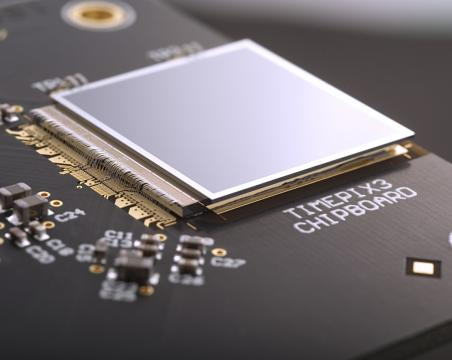
\includegraphics[width=7cm]{figures/timepix3.jpg}    
            \caption{Fotografie Timepix3 detektoru, osazeného na Timepix3 CERN chipboard \cite{medipix_from_medical_img_to_space}.}
        \end{subfigure}
        \hspace{0.1cm}
        \begin{subfigure}{7.0cm}
            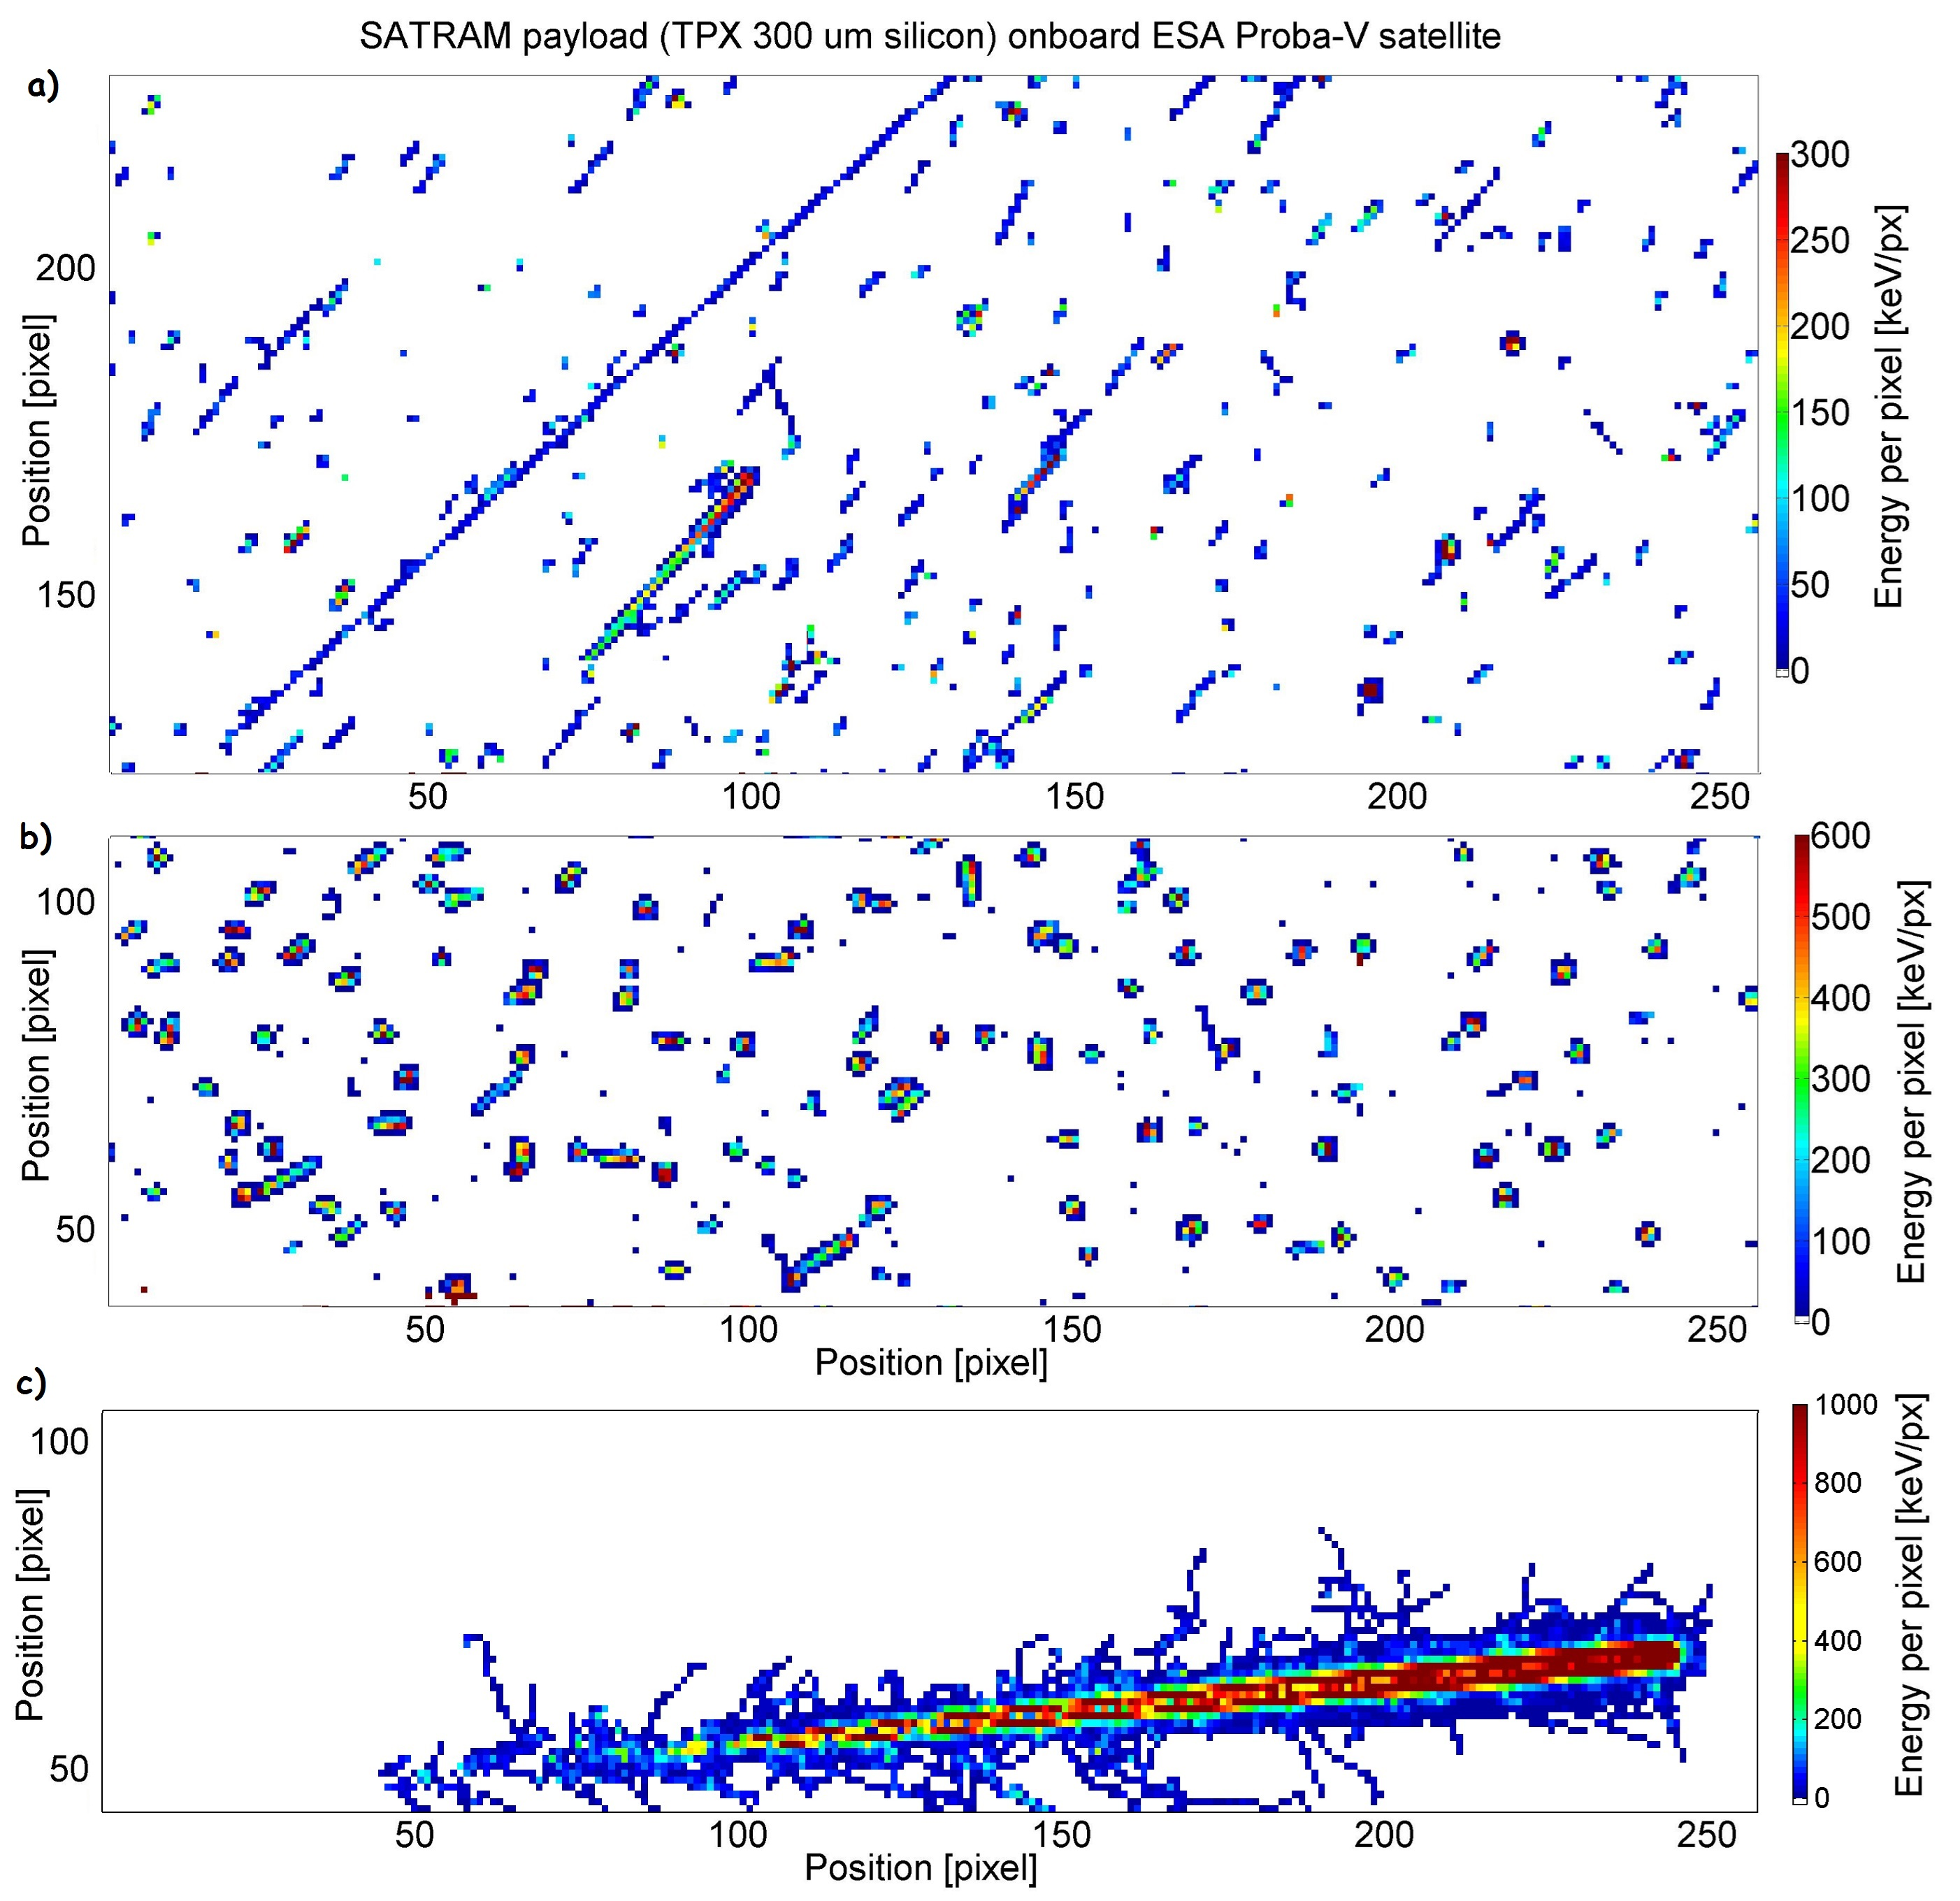
\includegraphics[width=7cm]{figures/timepix_data_satram.png}    
            \caption{Ukázka dat z detektoru Timepix, naměřených zařízením \textit{SATRAM} (z angl. \textit{Space Application of Timepix based Radiation Monitor}), které od roku 2013 obíhá Zemi na heliosynchronní kruhové polární dráze ve výšce \unit{820}{km} \cite{PlatkevicDisertace}.}
        \end{subfigure}
	\end{center}
    \caption{Detektor Timepix3 a vizualizace naměřeného vzorku dat.}
	\label{fig:master:frontend:detector_detail}
\end{figure}

Timepix3 detektor přináší oproti svému předchůdci několik výhod. Je schopný operovat i v kontinuálním módu, ve kterém je každý pixel detektoru schopný detekovanou událost ihned zpracovat, nezávisle na ostatních pixelech. Tím se téměř odstraňuje mrtvá doba detektoru, zvyšuje detekční účinnost, ale i zvyšuje datový tok z detektoru, jehož maximální teoretická hodnota je až $5.12 Gb/s$.

\section{Struktura práce}
Práce je strukturovaná do následujících kapitol:
\begin{itemize}
    
    \item \textbf{Kapitola} \ref{chap:detectors} - \nameref{chap:detectors}: V této kapitole bude čtenář seznámen se základními fyzikálními principy detekce ionizujícího záření v polovodiči, budou zde představeny hybridních částicové pixelové detektory rodiny \textit{Medipix}, včetně jejich módu, aspektů kalibrace a dostupných vyčítacích rozhraní.
    
    \item \textbf{Kapitola} \ref{chap:arch} - \nameref{chap:arch}: Tato kapitola se zabývá návrhem softwarové a hardwarové architektury systému Pixnet, budou zde popsány jeho komponenty a jejich vzájemné interakce. Rovněž zde bude diskutována škálovatelnost systému a budou zde uveden seznam použitých technologií, potřebných pro implementaci systému.
    
    \item \textbf{Kapitola} \ref{chap:handler} - \nameref{chap:handler}: V této kapitole bude čtenář seznámen s handlerem - komponentou systému Pixnet pro řízení jemu přiřazených detektorů.
    
    \item \textbf{Kapitola} \ref{chap:katherine} - \nameref{chap:katherine}: Tato kapitola je věnována vyčítacímu rozhraní \textit{Katherine} (zařízení pro řízení a vyčítání dat z detektoru \textit{Timepix3} s embedovaným počítačem, komunikující po ethernetu). Bude zde popsán návrh a implementace modulů, umožňující jeho integraci do systému Pixnet. Dále zde bude představen emulátor, který emuluje \textit{Katherine} na síťové vrstvě.
    
    \item \textbf{Kapitola} \ref{chap:master} - \nameref{chap:master}: V této kapitole bude představen master - centrální element systému Pixnet, který řídí handlery, přiřazuje jim detektory a umožňuje centralizované řízení detektorů.
    
    \item \todo testování...
    
    \item \textbf{Kapitola} \ref{chap:zaver} - \nameref{chap:zaver}: V závěru práce bude čtenář seznámen z dosaženými výsledky a plány na budoucí vývoj systému.

\end{itemize}